\subsection{Cross Sections as a function of Transverse Muon Momentum}
%Results in \tkiptmu 


Measurements of the differential cross section as a function of \tkiptmu \ for interactions on the nuclear targets are given in Fig.~\ref{fig:ptmu_xsec}.
 \tkiptmu \ is the magnitude of the muon momentum transverse to the beam direction in GeV/c.  The uncertainties broken down by source for both the absolute cross sections and the cross section ratios as a function of \tkiptmu\ can be found in Fig.~\ref{fig:xsec_err_muon_pt}.  

% tki_muon_pt xsec results
\begin{figure}[h]
	\centering
  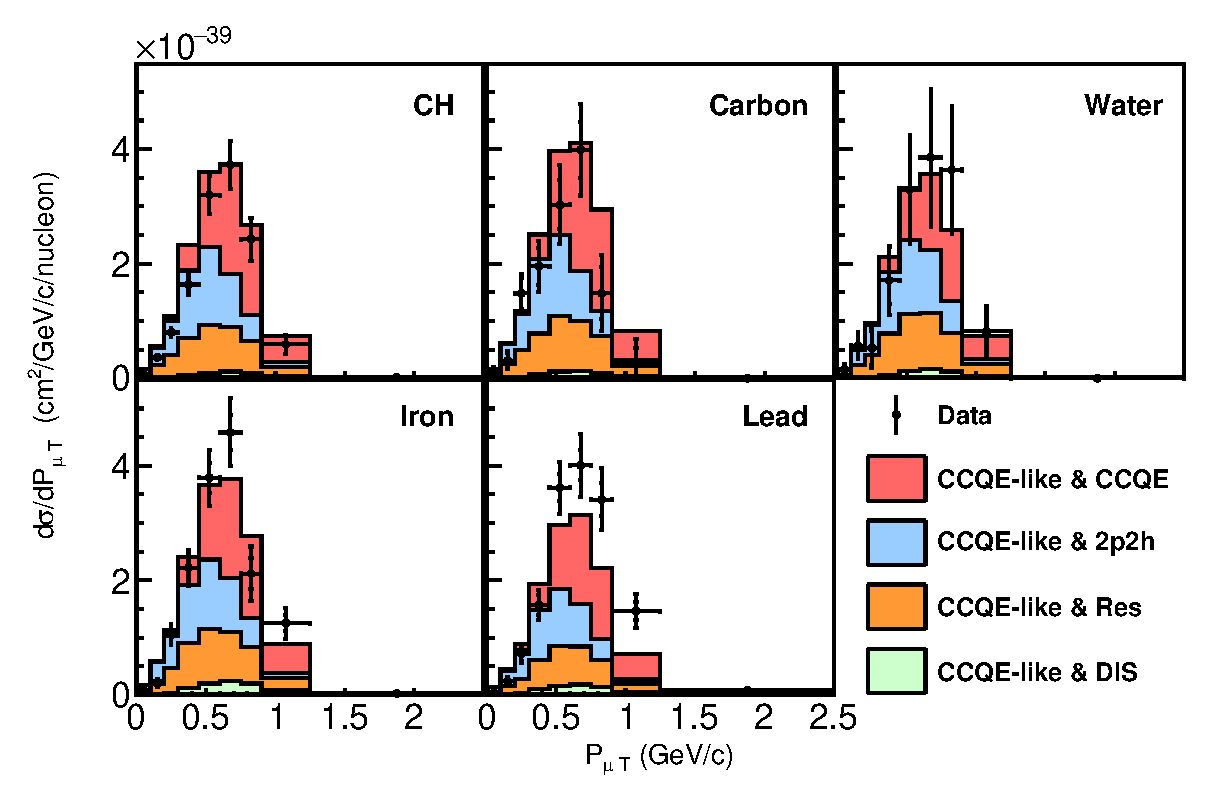
\includegraphics[width=\linewidth]{Figures/xsec_five_square/muon_pt.eps}
	\caption{The differential cross section as a function of \tkiptmu\ for CH, C, H$_{2}$O, Fe, and Pb targets, along with the predictions for the different quasielastic-like signal processes.}
	\label{fig:ptmu_xsec}
\end{figure}


Qualitatively, the MINERvA tune does a fairly good job describing the data for the smaller nuclear targets.  For the larger targets the data seem to have a slightly harder \tkiptmu \ spectrum.  This is pronounced for the data on the Pb target.

Figure~\ref{Figure:Gencompare_ptmu} shows comparisons of a range of models to 
the measured differential cross section as a function of \tkiptmu \ for the different targets. Qualitatively, 
For the smaller targets, the models cover the data fairly well, albeit with a spread.  For the larger nuclear targets, particularly for Pb, NEUT and the hN versions of GENIE exhibit higher cross sections than seen in the data.  Also on Pb, the data exhibit a slightly harder spectrum in \tkiptmu \ than seen in the models.
The \chisq\ between the cross sections and the models can be found in Table~\ref{tab:muonpt}.

% comparisons to generators muon_pt
\begin{figure}
    \centering            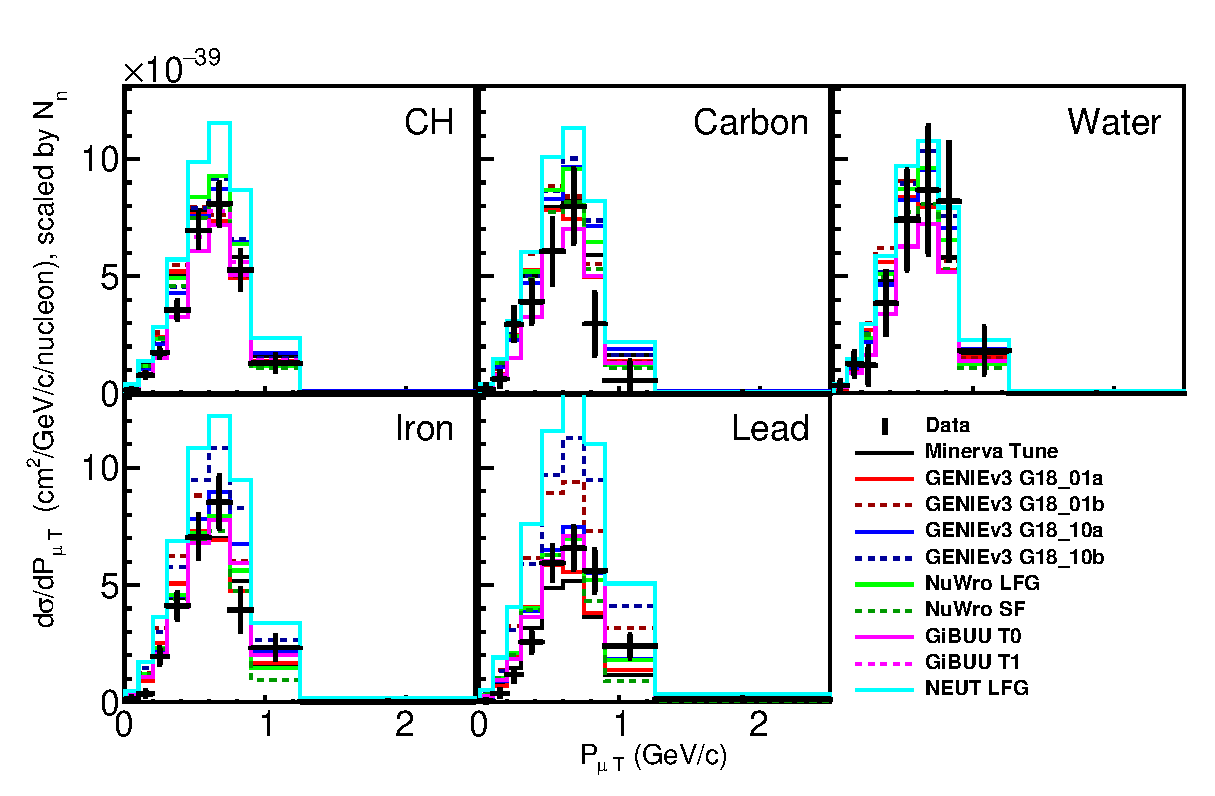
\includegraphics[width=\linewidth]{Figures/gencompare/muon_pt_5square.eps}
    \caption{\tkiptmu \ cross-section comparison for multiple targets }{Cross section measurements and predictions as a function of \tkiptmu\ for different targets and for a selection of different generator and model choices.}
    \label{Figure:Gencompare_ptmu}
\end{figure}


Figure~\ref{Figure:Gencompare_ptmu_ratio} shows the ratio of the 
of the differential cross section as a function of  \tkiptmu \ for each nuclear target to that for scintillator.  The harder \tkiptmu \ spectrum for Pb relative to scintillator is clearly shown as the ratio for the data grows as a function of \tkiptmu and that feature is not so much present for the models.
The \chisq\ between the cross section ratios and the models can be found in Table~\ref{tab:muonpt}.

\begin{figure}
    \centering
            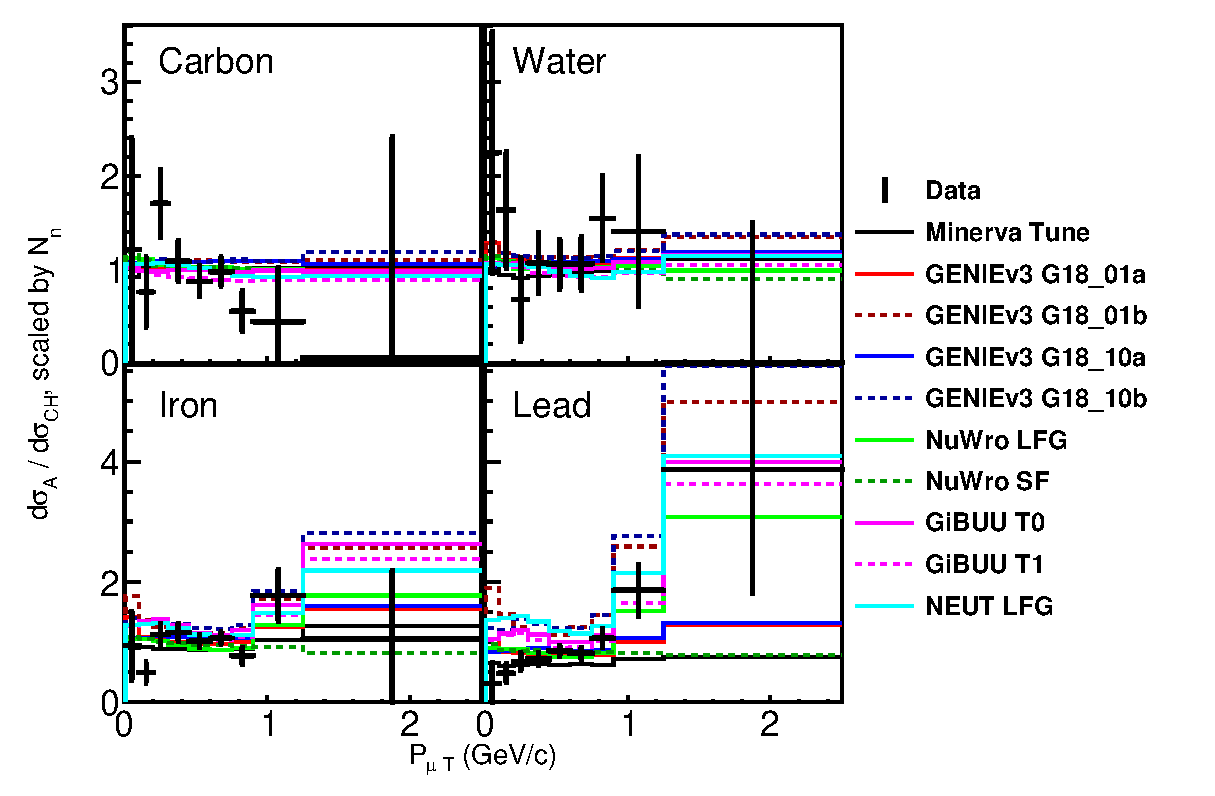
\includegraphics[width=\linewidth]{Figures/gencompare/muon_pt_4square.eps}
    \caption{\tkiptmu \ cross-section ratio generator comparison for multiple targets.   Changes to the FSI model (GENIE ``a'' to ``b'') in GENIE change the cross section ratio more than changes to the 2p2h model (GiBUU T0 to GiBUU T1) or changes to the initial state (GENIE 1 to GENIE 10) or (NuWro LFG to NuWro SF).  The changes to the ratio are most significant at high transverse muon momentum.}
        \label{Figure:Gencompare_ptmu_ratio}
\end{figure}

